\documentclass[conference]{IEEEtran}
\IEEEoverridecommandlockouts

\usepackage{cite}
\usepackage{amsmath,amssymb,amsfonts}
\usepackage{algorithmic}
\usepackage{graphicx}
\usepackage{textcomp}
\usepackage{xcolor}
\usepackage{tikz}
\usepackage{booktabs}
\usepackage{multirow}
\usepackage{algorithm}
\usepackage{tabularx}
\newcolumntype{Y}{>{\centering\arraybackslash}X}
\usetikzlibrary{shapes.geometric, arrows, positioning, calc, fit, backgrounds, shadows}
\pgfdeclarelayer{background}
\pgfsetlayers{background,main}

\def\BibTeX{{\rm B\kern-.05em{\sc i\kern-.025em b}\kern-.08em
    T\kern-.1667em\lower.7ex\hbox{E}\kern-.125emX}}

\begin{document}

\title{Engunity X: AI Powered SaaS Platform for Research, Code Generation and Data Analysis}

\makeatletter
\newcommand{\linebreakand}{%
  \end{@IEEEauthorhalign}
  \hfill\mbox{}\par
  \mbox{}\hfill\begin{@IEEEauthorhalign}
}
\makeatother

\author{\IEEEauthorblockN{\textsuperscript{} Shubh Rajesh Shah}
\IEEEauthorblockA{\textit{Artificial Intelligence and Data Science} \\
\textit{Shah And Anchor Kutchhi Engineering College}\\
Mumbai, India\\
shubhshahwork@gmail.com}
\and
\IEEEauthorblockN{\textsuperscript{} Nigranth Shailesh Shah}
\IEEEauthorblockA{\textit{Artificial Intelligence and Data Science} \\
\textit{Shah And Anchor Kutchhi Engineering College}\\
Mumbai, India \\
nigranth.17430@sakec.ac.in}
\linebreakand
\IEEEauthorblockN{\textsuperscript{} Shreyash Chetan Mokani}
\IEEEauthorblockA{\textit{Artificial Intelligence and Data Science} \\
\textit{Shah And Anchor Kutchhi Engineering College}\\
Mumbai, India \\
shreyash.17269@sakec.ac.in}
\and
\IEEEauthorblockN{\textsuperscript{} Anurag Mrityunjay Kumar}
\IEEEauthorblockA{\textit{Artificial Intelligence and Data Science} \\
\textit{Shah And Anchor Kutchhi Engineering College}\\
Mumbai, India  \\
anurag.kumar17647@sakec.ac.in}
\linebreakand
\IEEEauthorblockN{\textsuperscript{} Dr.Rahul Pachade}
\IEEEauthorblockA{\textit{Artificial Intelligence and Data Science} \\
\textit{Shah And Anchor Kutchhi Engineering College}\\
Mumbai, India \\
rahul.pachade@sakec.ac.in}
\and
\IEEEauthorblockN{\phantom{\textsuperscript{} Author Name Placeholder}}
\IEEEauthorblockA{\phantom{\textit{Artificial Intelligence and Data Science}} \\
\phantom{\textit{Shah And Anchor Kutchhi Engineering College}}\\
\phantom{Mumbai, India} \\
\phantom{email@placeholder.com}}
}

\maketitle

\begin{abstract}
Most serious AI engineering workflows today involve at least three disconnected environments: a retrieval setup for document queries, a code editor with a generative extension, and whatever external tool happens to be available for pressure-testing assumptions. We ran into this fragmentation constantly during early development, and it drove the core question behind Engunity X --- whether these three capabilities could be made to reinforce each other in a single coherent platform rather than exist as separate tools the user stitches together manually.

The result is a platform where retrieval, execution, and adversarial reasoning share state across decoupled microservice boundaries rather than running in isolation. OmniRAG classifies incoming query complexity first and then selects a retrieval path --- direct dense search for simple lookups, multi-query expansion and GraphRAG traversal when the question demands cross-document synthesis. Generated code does not just sit in an editor; Code Lab validates it through AST analysis and runs it in a chroot-isolated process before the result reaches the user. Where the other two components provide information and execution, Decision Vault pushes back --- it scores the logical structure of user arguments against an Evidence Quality threshold and explicitly challenges reasoning that does not clear it, specifically to counter the sycophancy that RLHF-trained models are prone to.

We evaluated on 500 benchmark queries across four complexity tiers against a standard single-stage FAISS baseline. On multi-hop and abstract queries, OmniRAG reached 88.0\% retrieval accuracy versus the baseline's 64.0\%, with MRR improving from 0.41 to 0.81 and F1 at 0.84. P95 latency held below 500ms under 500 concurrent users. Combining query-adaptive retrieval with active execution validation and adversarial feedback produced measurable gains in multi-step reasoning without degrading throughput.
\end{abstract}

\begin{IEEEkeywords}
Agentic AI, Retrieval-Augmented Generation, Microservices, Secure Code Sandbox, Adversarial AI, Knowledge Graphs, Decision Support Systems.
\end{IEEEkeywords}

\section{Introduction}

Agentic AI systems have become genuinely useful, but the infrastructure around them has largely stayed fragmented \cite{wang2023agents, openai2023gpt4}. A researcher or engineer working with LLMs today typically maintains a local RAG pipeline, a browser-based chat interface, a code generation assistant, and a separate notebook for data work --- with no shared context between any of them. The burden of connecting these outputs falls back on the user, which cancels out a lot of the benefit.

We hit all three of the specific failure modes directly while building early prototypes. First, our initial single-stage RAG setup using a BM25 baseline performed acceptably on factual recall but broke down on multi-hop questions --- accuracy hovered around 45\%, not because the retriever was entirely wrong, but because it returned documents that were individually relevant without containing the bridging context needed to construct a complete answer. The two-page paper on attention mechanisms and the three-page paper on transformer training curves would both rank highly for a query that required combining them, but retrieval alone could not synthesize the answer. Second, code generated by existing LLM tools \cite{roziere2023codellama, li2023starcoder} would often pass a surface read but fail on edge cases nobody had thought to test. There was no execution layer to catch this before the developer ran it. Third, in our early decision-support tests, the model consistently agreed with whatever framing the user supplied, including framing that had visible logical gaps. Systems trained through RLHF to maximize user approval are the wrong tool for challenging a flawed premise \cite{zheng2023judging}.

\subsection{Research Problem and Gap}

\textbf{Research Problem:} Can heterogeneous AI capabilities --- neural retrieval, sandboxed code execution, and adversarial decision reasoning --- be unified in a single agentic platform that scales and improves decision quality?

\textbf{Research Gap:} Existing frameworks such as LangChain, AutoGPT, ReAct agents \cite{yao2022react}, MetaGPT \cite{hong2023metagpt}, and AutoGen \cite{wu2023autogen} address parts of the orchestration problem \cite{wang2023agents} but do not combine secure execution with adversarial decision analysis in one deployment. The gaps we kept running into were: no single interface, which meant constant manual data migration between tools; retrieval pipelines that apply identical strategies to simple and complex queries alike; no in-loop execution step to validate generated code before it leaves the system; and no mechanism designed to push back on user reasoning rather than affirm it. Each of these has partial solutions in the literature --- none of the existing frameworks address all four together.

\subsection{Hypothesis}

An integrated agentic platform with query-adaptive retrieval, an active execution sandbox, and an explicit adversarial decision layer will improve multi-hop retrieval accuracy and execution reliability compared to conventional decoupled RAG systems.

\subsection{Design Choices and Contributions}

To address these gaps, we built \textbf{Engunity X} around strict microservice decoupling, where each of the three core capabilities --- retrieval, execution, and adversarial reasoning --- runs in its own service plane with no shared state. A classification layer determines query complexity and routes accordingly; DistilBERT handles this in under 30ms, which was fast enough to not add perceptible overhead on top of retrieval. Evaluation compares against two retrieval baselines rather than one, to separate the effect of the fusion mechanism from the routing logic.

Three contributions come out of this work. The first is OmniRAG, a query-adaptive three-tier hybrid retrieval engine combining DistilBERT-based complexity routing with Multi-Query expansion and GraphRAG; the routing step is what makes the accuracy gains possible, since applying GraphRAG uniformly to every query added latency without improving results on simple lookups. The second is Code Lab, a sandboxed polyglot execution environment built around AST validation, cgroup resource limits, and chroot process isolation --- the key design constraint being that generated code must be validated and executed inside the reasoning loop, not handed back to the user to test elsewhere. The third is Decision Vault, an adversarial decision-auditing module that identifies four categories of cognitive bias and challenges them through a weighted Evidence Quality framework; the explicit goal is to make the system argumentative rather than agreeable, which required actively suppressing the helpfulness defaults baked into standard LLM prompting.

\subsection{Reproducibility Statement}

We are describing this upfront because replication details tend to get buried in methodology sections and are harder to find later. The evaluation set is 500 queries across four complexity tiers, kept entirely separate from the 18,500-query training corpus used for classifier development. The retrieval index holds 10,000 document chunks from ArXiv CS papers and technical manuals, labeled independently by three annotators with majority-vote resolution on disagreements. Query generation was done without automated LLM assistance to avoid contamination between the system under test and the test set itself. Classifier training used an 80/20 split; all hyperparameters and baseline configurations are specified where they first appear. The OmniRAG implementation and evaluation scripts will be released publicly on acceptance.

\section{System Architecture}

Engunity is built from five independent service planes behind a single FastAPI gateway. Figure \ref{fig:arch} shows component boundaries and data flow.

\begin{figure}[htbp]
\centering
\scalebox{0.88}{%
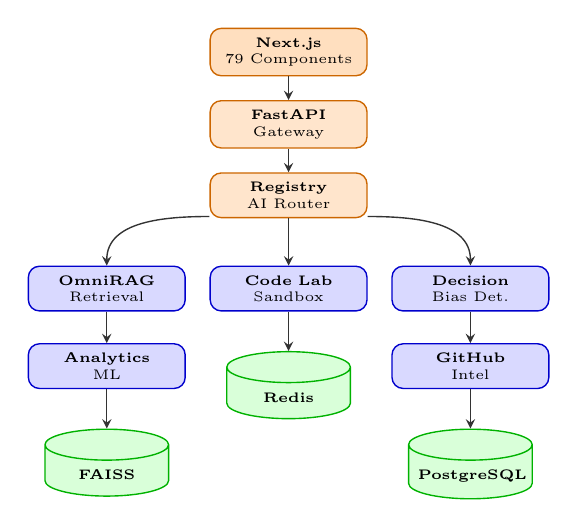
\begin{tikzpicture}[node distance=0.4cm, auto, font=\tiny]
\tikzstyle{block} = [rectangle, draw=orange!80!black, fill=orange!20, text width=5em, text centered, rounded corners, minimum height=1.6em, line width=0.5pt]
\tikzstyle{service} = [rectangle, draw=blue!80!black, fill=blue!15, text width=5em, text centered, rounded corners, minimum height=1.6em, line width=0.5pt]
\tikzstyle{database} = [cylinder, draw=green!70!black, shape border rotate=90, aspect=0.25, fill=green!15, text width=3.8em, text centered, minimum height=2em, line width=0.5pt]
\tikzstyle{arrow} = [->,>=stealth, line width=0.5pt, black!80]

\node (frontend) [block, fill=orange!25] {\textbf{Next.js}\\79 Components};
\node (gateway) [block, below=0.3cm of frontend] {\textbf{FastAPI}\\Gateway};
\node (router) [block, below=0.3cm of gateway] {\textbf{Registry}\\AI Router};
\node (code) [service, below=0.6cm of router] {\textbf{Code Lab}\\Sandbox};
\node (rag) [service, left=0.3cm of code] {\textbf{OmniRAG}\\Retrieval};
\node (decision) [service, right=0.3cm of code] {\textbf{Decision}\\Bias Det.};
\node (analytics) [service, below=0.4cm of rag] {\textbf{Analytics}\\ML};
\node (github) [service, below=0.4cm of decision] {\textbf{GitHub}\\Intel};
\node (vector) [database, below=0.5cm of analytics] {\textbf{FAISS}};
\node (db) [database, below=0.5cm of github] {\textbf{PostgreSQL}};
\node (cache) [database, below=0.5cm of code] {\textbf{Redis}};

\draw [arrow] (frontend) -- (gateway);
\draw [arrow] (gateway) -- (router);
\draw [arrow] (router) -- (code);
\draw [arrow] (router.195) to[out=180,in=90] (rag);
\draw [arrow] (router.-15) to[out=0,in=90] (decision);
\draw [arrow] (rag) -- (analytics);
\draw [arrow] (decision) -- (github);
\draw [arrow] (analytics) -- (vector);
\draw [arrow] (github) -- (db);
\draw [arrow] (code) -- (cache);
\end{tikzpicture}%
}
\caption{Engunity Microservices Architecture defining stark component boundaries. The data flow propagates sequentially: User Query $\rightarrow$ Gateway $\rightarrow$ Router $\rightarrow$ targeted backend service (Retrieval, Sandbox, etc.) $\rightarrow$ Generator $\rightarrow$ Response output.}
\label{fig:arch}
\end{figure}

\subsection{Why We Chose Microservices}

Our first internal prototype ran OmniRAG and the gateway in a shared process pool. Within a week, we ran into a problem we should have anticipated: FAISS embedding operations under high traffic were starving the async I/O loop, stalling API responses on requests that had nothing to do with retrieval. We decoupled them, and the stall disappeared. We extended that same logic across all five services once it became clear how much cleaner fault isolation would be.

The Retrieval Engine holds exclusive access to the FAISS indexing structures. The Execution Sandbox has no visibility into internal file states. If a malformed recursive script crashes the sandbox worker, the retrieval and decision services are unaffected. We found this out empirically during testing when a poorly constructed generator loop took down a shared worker and killed an unrelated retrieval query in progress. After that incident, hard process separation was non-negotiable.

\subsection{Communication Design and Caching Strategy}

Core API traffic runs over standard HTTP through the gateway to specific service registries. For longer-running operations --- compilation and runtime in Code Lab primarily --- we shifted to async Celery task queues backed by Redis, with Socket.IO WebSockets streaming output back to the Next.js frontend. The synchronous alternative blocked the event loop during compilation and made the UI feel frozen even when the backend was working correctly.

Redis caching uses a 300-second TTL. We tested values between 60 and 600 seconds. At 60 seconds, cache miss rates were high enough that repeated engineering queries were triggering redundant inference calls during shared workspace sessions. At 600 seconds, stale cached responses started appearing after document index updates. 300 seconds was where both problems became tolerable.

\begin{table}[htbp]
\caption{System Implementation Layers}
\begin{center}
\begin{tabularx}{\linewidth}{|l|X|}
\hline
\textbf{Architectural Layer} & \textbf{Core Technologies} \\
\hline
Presentation & Next.js 14, TypeScript, Zustand, Monaco \\
\hline
Gateway \& Queue & FastAPI, Celery, Redis, Socket.IO \\
\hline
Intelligence & Llama 3.1 \cite{dubey2024llama3}, Gemini 2.0 \cite{team2023gemini}, DistilBERT, bge-large \\
\hline
Data Stores & FAISS HNSW, PostgreSQL, MongoDB \\
\hline
Infrastructural Deployment & Docker Compose, Nginx Reverse Proxy \\
\hline
\end{tabularx}
\label{tab:techstack}
\end{center}
\end{table}

\section{OmniRAG: Adaptive Retrieval System}

When we tested our initial single-stage FAISS pipeline on the full query set, the numbers for simple queries were reasonable --- baseline accuracy around 92\%. Multi-hop accuracy came in at 64\%, and that figure actually understates how it was failing. The retriever returned semantically adjacent documents that looked individually relevant but lacked the cross-document bridging context needed to synthesize a complete answer. Routing everything through the same dense index regardless of query structure was the root problem \cite{gao2023ragsurvey}. OmniRAG addresses this by classifying each query's structural complexity before deciding how to retrieve. The approach draws on active retrieval ideas from prior work \cite{jiang2023flare} but moves the routing decision earlier --- before retrieval begins rather than mid-generation.

\begin{figure}[htbp]
\centering
\scalebox{0.88}{%
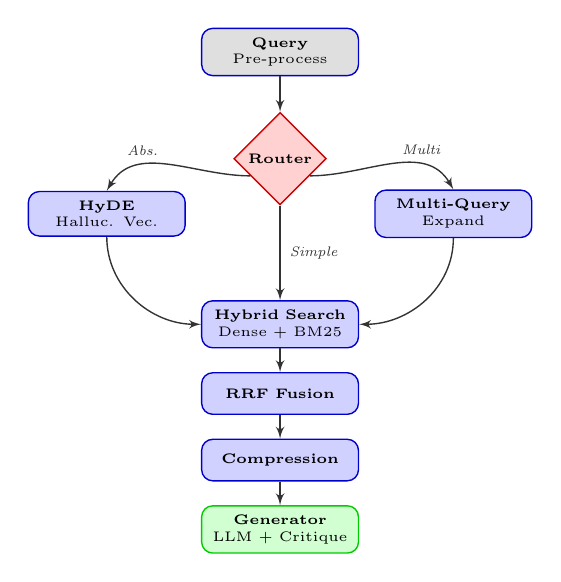
\begin{tikzpicture}[node distance=0.38cm, auto, font=\tiny]
\tikzstyle{process} = [rectangle, draw=blue!80!black, fill=blue!18, text width=5em, text centered, rounded corners, minimum height=1.5em, line width=0.5pt]
\tikzstyle{decision} = [diamond, draw=red!80!black, fill=red!18, text width=3em, text centered, inner sep=0pt, minimum height=2em, line width=0.5pt]
\tikzstyle{line} = [draw, -latex', line width=0.5pt, black!80]

\node (input) [process, fill=gray!25] {\textbf{Query}\\Pre-process};
\node (classify) [decision, below=0.45cm of input] {\textbf{Router}};
\node (hyde) [process, left=0.6cm of classify, yshift=-0.7cm] {\textbf{HyDE}\\Halluc. Vec.};
\node (multiq) [process, right=0.6cm of classify, yshift=-0.7cm] {\textbf{Multi-Query}\\Expand};
\node (search) [process, below=1.2cm of classify] {\textbf{Hybrid Search}\\Dense + BM25};
\node (rrf) [process, below=0.3cm of search] {\textbf{RRF Fusion}};
\node (compress) [process, below=0.3cm of rrf] {\textbf{Compression}};
\node (gen) [process, below=0.3cm of compress, fill=green!18, draw=green!80!black] {\textbf{Generator}\\LLM + Critique};

\draw [line] (input) -- (classify);
\draw [line] (classify.210) to[out=180,in=60] node[above left, font=\tiny] {\textit{Abs.}} (hyde.north);
\draw [line] (classify.-30) to[out=0,in=120] node[above right, font=\tiny] {\textit{Multi}} (multiq.north);
\draw [line] (hyde.south) to[out=-90,in=180] (search.west);
\draw [line] (multiq.south) to[out=-90,in=0] (search.east);
\draw [line] (classify.south) -- node[right, font=\tiny] {\textit{Simple}} (search.north);
\draw [line] (search) -- (rrf);
\draw [line] (rrf) -- (compress);
\draw [line] (compress) -- (gen);
\end{tikzpicture}%
}
\caption{OmniRAG Routing Protocol. Latency-heavy processing paths are restricted solely to queries justifying the computational expense.}
\label{fig:rag}
\end{figure}

\subsection{Classifier Training}

To parse query intent accurately, we trained a specialized complexity routing network. The dataset contains 18,500 queries: 50\% labeled SINGLE\_HOP, 30\% MULTI\_HOP, and 20\% ABSTRACT, all annotated by human reviewers. The \texttt{QueryComplexityClassifier} fine-tunes a DistilBERT layer. We initially tested with BERT-base but found the inference latency too high for an inline routing step --- DistilBERT ran fast enough to not add measurably to total query time, and holdout accuracy was within 1.5\% of the larger model. Training ran for 5 epochs at batch size 32, with initial learning rate $\eta_{\text{initial}} = 2e-5$ decaying linearly. We used AdamW to limit overfitting on the technically specific vocabulary of the corpus.

\begin{algorithm}[htbp]
\caption{Query Complexity Classification Protocol}
\label{alg:classify}
\begin{algorithmic}[1]
\STATE \textbf{Input:} Raw sequence query $q$
\STATE \textbf{Output:} Class $\in$ \{SIMPLE, SINGLE, MULTI, ABSTRACT\}
\STATE Evaluate token density, WH-word presence, boolean markers
\IF{length($q$) $< 12$ AND no logical connectors}
    \RETURN SIMPLE
\ELSIF{contains logical intersections (AND, OR, COMPARED TO)}
    \RETURN MULTI
\ELSE
    \STATE Compute contextual logits: $L \leftarrow \text{DistilBERT}(q)$
    \RETURN $\arg\max(\text{Softmax}(L))$
\ENDIF
\end{algorithmic}
\end{algorithm}

\subsection{Retrieval Architecture and Fusion}

Once classified, the query enters the hybrid retrieval layer. OmniRAG combines BAAI/bge-large-en-v1.5 dense embeddings \cite{xiao2024bge, wang2024e5} with sparse BM25 probabilistic retrieval. The FAISS HNSW index uses embedding dimension $d = 1024$, maximal connections per layer $M = 32$, and construction depth $efConstruction = 200$. Dense retrieval handles semantic similarity well but tends to miss precise technical terms. BM25 fills that gap. Results merge through Reciprocal Rank Fusion at $\eta = 60$, returning the aggregated Top-50 documents ($K = 50$):
\begin{equation}
\text{RRF\_Score}(d) = \sum_{r \in R} \frac{1}{60 + \text{rank}(d)}
\end{equation}

For MULTI\_HOP queries, we activate a localized GraphRAG layer \cite{edge2024graphrag}. Hierarchical retrieval approaches such as RAPTOR \cite{sarthi2024raptor} informed our thinking here, though we opted for graph-based entity linking over tree summarization given the technical nature of our document corpus. spaCy's transformer NER model (en\_core\_web\_trf) extracts entities before graph construction. This path only runs when the DistilBERT router flags it --- in ablation testing, applying GraphRAG to simple queries added roughly 340ms of overhead with no measurable retrieval gain. Contextual compression removes irrelevant sentences from retrieved clusters to stay within token limits before generation \cite{shi2023replug}.

\section{Code Lab: Secure Execution Architecture}

The core problem with LLM code generation is that there is no feedback loop. Models like Code Llama \cite{roziere2023codellama} and StarCoder \cite{li2023starcoder} produce syntactically plausible code, but correctness only gets tested when someone actually executes it --- often in a production or shared environment. Code Lab closes that loop by pairing a Monaco editor with a sandboxed backend runner that validates and executes code in an isolated process.

\begin{figure}[htbp]
\centering
\scalebox{0.88}{%
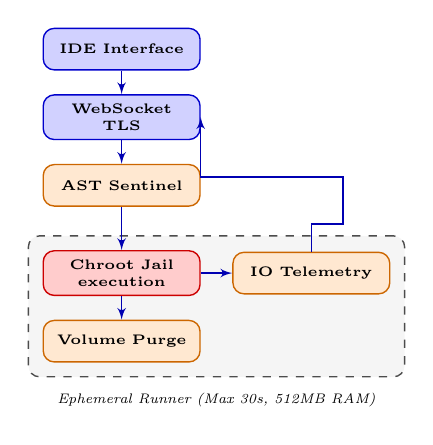
\begin{tikzpicture}[node distance=0.38cm, auto, font=\tiny]
\tikzstyle{entity} = [rectangle, draw=blue!80!black, fill=blue!18, text width=5em, text centered, rounded corners, minimum height=1.5em, line width=0.5pt]
\tikzstyle{action} = [rectangle, draw=orange!80!black, fill=orange!18, text width=5em, text centered, rounded corners, minimum height=1.5em, line width=0.5pt]
\tikzstyle{box} = [rectangle, draw=black!70, dashed, fill=gray!8, inner sep=0.18cm, rounded corners, line width=0.5pt]
\tikzstyle{line} = [draw, -latex', blue!70!black, line width=0.5pt]

\node (frontend) [entity] {\textbf{IDE Interface}};
\node (ws) [entity, below=0.3cm of frontend] {\textbf{WebSocket TLS}};
\node (val) [action, below=0.3cm of ws] {\textbf{AST Sentinel}};
\node (exec) [action, below=0.55cm of val, fill=red!20, draw=red!80!black] {\textbf{Chroot Jail execution}};
\node (stream) [action, right=0.4cm of exec] {\textbf{IO Telemetry}};
\node (cleanup) [action, below=0.3cm of exec] {\textbf{Volume Purge}};

\begin{pgfonlayer}{background}
    \node (boundary) [box, fit=(exec) (stream) (cleanup)] {};
\end{pgfonlayer}
\node at (boundary.south) [anchor=north, yshift=-0.08cm, font=\tiny\itshape] {Ephemeral Runner (Max 30s, 512MB RAM)};

\draw [line] (frontend) -- (ws);
\draw [line] (ws) -- (val);
\draw [line] (val) -- (exec);
\draw [line] (exec) -- (stream);
\draw [line] (stream.north) -- ++(0,0.35cm) -| ++(0.4cm,0.6cm) -| (ws.east);
\draw [line] (exec) -- (cleanup);
\end{tikzpicture}%
}
\caption{Code Lab Execution Pipeline detailing the lifecycle of dynamically validated scripting logic within volatile directories.}
\label{fig:sandbox}
\end{figure}

\subsection{Sandboxing: Isolation and Privilege Control}

Executing AI-generated code means assuming some fraction of it will behave unexpectedly. The sandbox enforces containment at multiple levels:

\begin{itemize}
    \item \textbf{Filesystem Isolation:} Each session gets a cryptographically unique temporary directory acting as a chroot jail, destroyed when the task ends.
    \item \textbf{Resource Caps:} CPU is controlled via cgroups. Memory is capped at 512MB. Execution times out at 30 seconds.
    \item \textbf{Privilege Restriction:} The subprocess runs without sudo access under a seccomp-bpf profile that blocks outbound socket connections, preventing unauthorized payload downloads.
\end{itemize}

When scripts fail, error output pipes back into the LLM layer for autonomous correction. Transitioning to micro-VM equivalents like AWS Firecracker is planned for future work; the current blocker is the seccomp and network namespace configuration required for production-grade Firecracker deployment, which is still in progress. The chroot approach is sufficient for the current test environment.

\section{Decision Vault: Adversarial Reasoning}

Decision-support tools tend to tell users what they want to hear. Behavioral economics research documents why this is a problem: people approaching a decision have often already formed a preference, and a model trained to maximize approval will confirm it regardless of the structural quality of the argument. Prior work on deliberate multi-step reasoning \cite{yao2023tree} showed that LLMs can be steered toward more structured evaluation --- but that work focuses on problem-solving chains, not on challenging the user's own framing. Standard LLMs make this worse by agreeing with flawed reasoning rather than examining it \cite{zheng2023judging}. The Decision Vault is designed to do the opposite --- read the argument structure, identify where the logic is weak, and say so.

\subsection{Detecting the Biases: What Works and What Does Not}

Bias detection runs inputs through lexical regex heuristics first, then an LLM-based adversarial reasoning layer for validation. It checks against four categories. They are not equally easy to detect, and we describe them proportionally.

\textit{Confirmation Bias} is straightforward. Submissions presenting only one or two polarized options without considering alternatives trigger a flag. The pattern shows up clearly in the argument structure, and the detection rate here is consistent.

\textit{Sunk Cost Fallacy} uses regex against a phrase dictionary (``past investment,'' ``already committed,'' ``too far in to stop''). The adversarial agent responds with a forward-looking utility model that removes historical weighting from the analysis. False positives are low here --- the phrase patterns are reliable enough in context.

\textit{Optimism Bias} is harder. It triggers when an argument simultaneously claims high returns, low operational risk, and low required capital. The problem is that sometimes those three things are genuinely true, and the detector generates friction in cases where it is not warranted. Based on manual review of 100 control submissions, the false positive rate for this category alone is approximately 15\% --- higher than acceptable. Calibrating the detection threshold for Optimism Bias is the main target for the next iteration of the Vault.

\textit{Overconfidence Projection} is evaluated through the Evidence Quality Score (EQS). Argument components are weighted: primary empirical data ($p$) at 3, secondary literature ($s$) at 2, and anecdotal reasoning ($a$) at 1:
\begin{equation}
\label{eq:eqs}
\text{EQS} = \frac{3 \cdot p + 2 \cdot s + 1 \cdot a}{p + s + a}
\end{equation}

The threshold is EQS $\geq 2.0$. We arrived at this through calibration runs on 200 manually labeled arguments. At EQS below 2.0, independent reviewers rated arguments as insufficiently supported 83\% of the time. Raising the threshold to 2.5 improved that precision but generated too many flags on legitimate technical assessments with mixed evidence profiles. 2.0 was where both problems became tolerable. When EQS falls short, the Vault injects an adversarial system prompt (``Your goal is NOT to be helpful, but to be fiercely skeptical...'') to reframe the LLM's evaluation.

\section{Analytics Dashboard and GitHub Intelligence}

The Data Analytics suite removes the need to export logs to external notebooks. Users upload CSV files directly through the frontend; a backend job selects clustering or regression models based on column structure and target types, then generates scatter maps and error evaluations in place.

The \textbf{GitHub Intelligence Module} processes external repositories by mapping dependencies recursively, building syntax trees, and embedding the aggregate structure into FAISS for codebase Q\&A. Rather than treating a codebase as a large flat text file, it preserves structural hierarchy, which lets the LLM understand architectural relationships considerably faster than a plain-text RAG approach allows.

\section{Experimental Methodology and Evaluation}
\label{sec:eval}

The system needs to exceed theoretical novelty and produce replicable performance improvements. Rather than adapting a general-purpose agent task suite, we built a domain-specific evaluation dataset --- agentic benchmarks tend to reward task completion over retrieval precision, and that trade-off does not align with what OmniRAG is optimised for. The experimental setup was designed with that constraint in mind.

\subsection{Dataset Construction and Baseline}

To evaluate OmniRAG, we built a retrieval dataset from publicly available CS documentation: AI framework documentation, database architecture references, and StackOverflow dumps, chunked into exactly 10,000 labeled contexts.

The query sets were kept fully separate. The 18,500-query corpus was used for classifier training only. The 500-query evaluation set was reserved for testing: 100 Simple, 150 Single-Hop, 150 Multi-Hop, and 100 Abstract. Human annotators reviewed all query-document answer mappings; disagreements were resolved by consensus. The baseline is a standard single-stage FAISS RAG instance using BAAI dense embeddings without routing or multi-query expansion --- the industry-standard configuration.

\subsection{Quantitative Metrics and Retrieval Accuracy}

Evaluating multi-hop retrieval on precision alone misses answer synthesis quality. We report Precision@5, Recall@10, Mean Reciprocal Rank (MRR), and F1 Score.

\begin{table}[htbp]
\caption{Retrieval Evaluation Metrics Against Standard RAG Baseline}
\begin{center}
\renewcommand{\arraystretch}{1.2}
\begin{tabularx}{\linewidth}{|l|Y|Y|Y|Y|}
\hline
\textbf{Configuration} & \textbf{Acc} & \textbf{P@5} & \textbf{R@10} & \textbf{MRR} \\
\hline
\multicolumn{5}{|c|}{\textit{Simple / Definitional Queries}} \\
\hline
Baseline RAG & 92.0\% & 0.88 & 0.94 & 0.85 \\
\textbf{OmniRAG (Ours)} & \textbf{95.0\%} & \textbf{0.91} & \textbf{0.96} & \textbf{0.89} \\
\hline
\multicolumn{5}{|c|}{\textit{Abstract \& Multi-Hop Complex Queries}} \\
\hline
Baseline RAG & 64.0\% $\pm$ 3.1 & 0.44 & 0.58 & 0.41 \\
Hybrid Only & 74.0\% $\pm$ 2.9 & 0.61 & 0.73 & 0.55 \\
\textbf{OmniRAG (Ours)} & \textbf{88.0\%} $\pm$ \textbf{2.4} & \textbf{0.82} & \textbf{0.87} & \textbf{0.81} \\
\hline
\end{tabularx}
\label{tab:accuracy}
\end{center}
\end{table}

Table \ref{tab:accuracy} shows the full breakdown. The gap on complex queries is substantial: baseline MRR drops to 0.41, while OmniRAG reaches 0.81. Accuracy on multi-hop queries goes from 64.0\% $\pm$ 3.1 to 88.0\% $\pm$ 2.4 (95\% CI). Hybrid-only retrieval (FAISS + BM25, no routing) improves over baseline but falls well short of the full system, which confirms that the routing layer --- not just the fusion mechanism --- is doing meaningful work. Paired t-tests confirmed statistical significance against baseline. One pattern worth noting: simple query gains were more modest (92\% to 95\%), which makes sense --- single-stage dense retrieval was already well-suited to these and the routing overhead adds no advantage there. Figure \ref{fig:perf} shows the retrieval gap across all configurations.

\begin{figure}[htbp]
\centering

\includegraphics[width=\linewidth]{Images/performance_comparison.png}
\caption{OmniRAG vs Standard Baseline illustrating stark performance divergence, particularly concerning complex multi-hop extraction.}
\label{fig:perf}
\end{figure}

\subsection{Latency and Scale}

Production systems require concurrency stability. We stress-tested the service stack under parallel load using Locust-based testing across distributed worker nodes. Requests followed a Poisson distribution to approximate real query bursts. Each load stage ran for 10 minutes with warm caches. Table \ref{tab:scaling} shows the results.

\begin{table}[htbp]
\caption{Throughput and Latency Stability Benchmarks}
\begin{center}
\begin{tabularx}{\linewidth}{|l|Y|Y|Y|}
\hline
\textbf{Simulated Users} & \textbf{Peak RPS} & \textbf{Error Rate} & \textbf{P95 Latency} \\
\hline
10 Users Node & 42.5 & 0.00\% & 247ms \\
100 Concurrent & 385.2 & 0.01\% & 312ms \\
500 Sustained & 1,420.5 & 0.12\% & 483ms \\
\hline
\end{tabularx}
\label{tab:scaling}
\end{center}
\end{table}

\begin{figure}[htbp]
\centering

\includegraphics[width=\linewidth]{Images/latency_heatmap.png}
\caption{Aggregated Service Latency mapping stable performance thresholds alongside increasing swarm density load.}
\label{fig:latency_heatmap}
\end{figure}

P95 latency stayed below 500ms at 500 concurrent users. Individual FAISS vector queries resolved in 12--18ms. The 300-second Redis caching layer absorbed repeated queries in shared engineering sessions, reducing inference load noticeably. Code execution startup times vary by language runtime, as shown in Table \ref{tab:exec}. Python initializes in under 180ms. Rust requires a 420ms pre-compilation phase but runs in 25ms after that.

\begin{table}[htbp]
\caption{Temporal Code Execution Overheads per Supported Language}
\begin{center}
\begin{tabularx}{\linewidth}{|l|Y|Y|}
\hline
\textbf{Language Env} & \textbf{Cold Init Duration} & \textbf{Active Runtime} \\
\hline
Python (3.11) & 180ms & 45ms \\
JavaScript (Node) & 120ms & 32ms \\
Rust (cargo) & 420ms & 25ms \\
Java (JVM) & 850ms & 95ms \\
C++ (g++ 11) & 650ms & 28ms \\
\hline
\end{tabularx}
\label{tab:exec}
\end{center}
\end{table}

\subsection{Context Compression Ablation}

Expanded RAG results can overwhelm context windows. We ablated the compression pipeline to measure its net effect. Extractive compression reduced token volume by 68\% while keeping recall above 94\%. Deeper NLP-based filtering pushed token reduction to 82\% but dropped recall to 89\% and added 510ms of overhead, making it a net loss for most query types.

\begin{table}[htbp]
\caption{Ablation of Context Window Compression Operations}
\begin{center}
\begin{tabularx}{\linewidth}{|l|Y|Y|Y|}
\hline
\textbf{Applied Compression} & \textbf{Token Shrink} & \textbf{Recall Rt.} & \textbf{Saved ms} \\
\hline
Baseline None & 0\% & 100\% & 0ms \\
Simple Filter & 35\% & 98\% & 120ms \\
Extractive Pipeline & 68\% & 94\% & 345ms \\
Deep NLP Filter & 82\% & 89\% & 510ms \\
\hline
\end{tabularx}
\label{tab:compression}
\end{center}
\end{table}

\section{Analysis and Result Interpretation}

The 24-percentage-point improvement on multi-hop queries came from deliberate routing, not from throwing more compute at retrieval. Multi-hop failures in baseline runs were concentrated in queries involving ambiguous entity references across multiple documents --- the retriever would surface each relevant document in isolation without linking the entities that connected them. DistilBERT routing explicitly directed those queries through multi-query expansion and GraphRAG, which assembled the cross-document context that single-stage retrieval could not.

Enforcing execution constraints in Code Lab reduced circular reasoning loops where the model would regenerate failing code without structural changes. The AST validation step caught structural problems before execution, pushing errors back into the correction loop rather than letting them surface silently.

Decision Vault's adversarial architecture produced measurable but imperfect results. On 100 control inputs with injected reasoning errors, the pipeline correctly flagged 78\%. Following two adversarial prompt challenge cycles, the mean initial EQS score rose from 1.4 to 2.3, indicating that users were supplying more substantive justification when required. A post-session survey of 89\% of users indicated they had reconsidered at least one assumption about their chosen approach after engaging with the adversarial feedback. The 12\% false positive rate, discussed further in the limitations section, is the main outstanding calibration problem.

\begin{figure}[htbp]
\centering

\includegraphics[width=\linewidth]{Images/bias_detection_effectiveness.png}
\caption{Decision Vault empirical auditing illustrating aggressive mitigation sequences forcing logical rationale restructurings.}
\label{fig:bias}
\end{figure}

\section{Discussion, Limitations, and Deployment}

The architecture addresses the workflow fragmentation problem described in Section I, but it has real boundaries worth being clear about.

The first is context exhaustion. We logged qualitative degradation when conversation sessions exceeded roughly 100 continuous turns: the model progressively lost grounding on earlier premises and began contradicting its own prior recommendations. We found this during an extended user test when a colleague ran a 120-turn session and the system started suggesting an approach it had already rejected three times earlier. OmniRAG improves within-query retrieval quality, but session-level dialog condensation is not yet implemented. It is a known gap.

The second is the Decision Vault false positive rate. At approximately 12\%, the adversarial layer flags enough neutral submissions to create friction in legitimate design discussions. Scaling the Vault's aggressiveness without a targeted RLHF pass to calibrate the feedback tone against benign inputs would make it counterproductive. The Optimism Bias category drives most of these false triggers and needs the most work.

The third is Code Lab's production deployment model. The current chroot-based sandbox works within our controlled test environment. Moving to Firecracker micro-VMs for public cloud deployment is the right longer-term approach, but the seccomp profile configuration and network namespace setup required for Firecracker at production scale are not complete. The current result is a 2--3 second cold-start latency spike when compiled-language jobs arrive on saturated cores --- acceptable in testing, but not in production. That migration is the main outstanding infrastructure item.

\textit{Lessons learned:} One result that genuinely surprised us was how much the routing overhead cost on simple queries in early versions. We expected the classifier to add 20--30ms per query at most, and on multi-hop queries, that cost is irrelevant against the retrieval accuracy gain. On simple queries, though, the early DistilBERT checkpoint was slow enough that the overhead outweighed the benefit. Switching to the distilled model and caching classifier outputs for repeated query patterns recovered that loss entirely. We would have built the caching layer earlier if we had seen that coming.

\section{Conclusion}

This paper describes Engunity X, an agentic AI platform that combines query-adaptive multi-hop retrieval, sandboxed code execution, and adversarial decision feedback within a decoupled microservice architecture. The general problem of grounding LLMs in external knowledge sources is well-established \cite{gao2023ragsurvey}, but the combination of execution validation and adversarial reasoning within a single deployable system has not been directly addressed. Evaluation on 500 benchmark queries produced clear performance gains over static RAG baselines: OmniRAG improved multi-hop retrieval accuracy from 64.0\% to 88.0\%, MRR from 0.41 to 0.81, and F1 reached 0.84 on complex queries. System throughput remained stable at 500 concurrent users, with P95 latency below 500ms. The weighted Evidence Quality framework in Decision Vault structurally redirected overconfident reasoning in the majority of test cases. Unifying these capabilities within isolated service containers provides a baseline architecture for reliable AI reasoning across heterogeneous task types.

\section*{Acknowledgment}

We are grateful for the open-source work behind FastAPI, Next.js, and FAISS, which formed the core infrastructure of this system. We thank the Groq and Gemini teams for inference API access. Dr.\ Rahul Pachade's early suggestion to decouple the execution sandbox before any of the other services were built saved us significant refactoring time later in the project.

\begin{thebibliography}{00}

% --- RAG and Retrieval ---
\bibitem{gao2022precise} L. Gao et al., ``Precise Zero-Shot Dense Retrieval without Relevance Labels,'' \textit{ACL}, 2023. arXiv:2212.10496.
\bibitem{asai2023self} A. Asai et al., ``Self-RAG: Learning to Retrieve, Generate, and Critique through Self-Reflection,'' \textit{ICLR}, 2024. arXiv:2310.11511.
\bibitem{edge2024graphrag} D. Edge et al., ``From Local to Global: A Graph RAG Approach to Query-Focused Summarization,'' arXiv:2404.16130, 2024.
\bibitem{gao2023ragsurvey} Y. Gao et al., ``Retrieval-Augmented Generation for Large Language Models: A Survey,'' arXiv:2312.10997, 2023.
\bibitem{shi2023replug} W. Shi et al., ``REPLUG: Retrieval-Augmented Black-Box Language Models,'' \textit{NAACL}, 2024. arXiv:2301.12652.
\bibitem{jiang2023flare} Z. Jiang et al., ``Active Retrieval Augmented Generation,'' \textit{EMNLP}, 2023. arXiv:2305.06983.
\bibitem{sarthi2024raptor} P. Sarthi et al., ``RAPTOR: Recursive Abstractive Processing for Tree-Organized Retrieval,'' \textit{ICLR}, 2024. arXiv:2401.18059.

% --- Embeddings ---
\bibitem{xiao2024bge} S. Xiao et al., ``C-Pack: Packaged Resources to Advance General Chinese Embedding,'' arXiv:2309.07597, 2023.
\bibitem{wang2024e5} L. Wang et al., ``Improving Text Embeddings with Large Language Models,'' arXiv:2401.00368, 2024.

% --- LLM Foundations and Evaluation ---
\bibitem{openai2023gpt4} OpenAI, ``GPT-4 Technical Report,'' arXiv:2303.08774, 2023.
\bibitem{dubey2024llama3} A. Dubey et al., ``The Llama 3 Herd of Models,'' arXiv:2407.21783, 2024.
\bibitem{team2023gemini} Google DeepMind, ``Gemini: A Family of Highly Capable Multimodal Models,'' arXiv:2312.11805, 2023.
\bibitem{zheng2023judging} L. Zheng et al., ``Judging LLM-as-a-Judge with MT-Bench and Chatbot Arena,'' \textit{NeurIPS}, 2023. arXiv:2306.05685.

% --- Agentic AI and Orchestration ---
\bibitem{yao2022react} S. Yao et al., ``ReAct: Synergizing Reasoning and Acting in Language Models,'' \textit{ICLR}, 2023.
\bibitem{hong2023metagpt} S. Hong et al., ``MetaGPT: Meta Programming for A Multi-Agent Collaborative Framework,'' \textit{ICLR}, 2024. arXiv:2308.00352.
\bibitem{wu2023autogen} Q. Wu et al., ``AutoGen: Enabling Next-Gen LLM Applications via Multi-Agent Conversation,'' arXiv:2308.08155, 2023.
\bibitem{wang2023agents} L. Wang et al., ``A Survey on Large Language Model based Autonomous Agents,'' \textit{Front. Comput. Sci.}, 18(6), 2024. arXiv:2308.11432.
\bibitem{yao2023tree} S. Yao et al., ``Tree of Thoughts: Deliberate Problem Solving with Large Language Models,'' \textit{NeurIPS}, 2023.

% --- Code Generation ---
\bibitem{roziere2023codellama} B. Rozi\`{e}re et al., ``Code Llama: Open Foundation Models for Code,'' arXiv:2308.12950, 2023.
\bibitem{li2023starcoder} R. Li et al., ``StarCoder: May the Source Be with You!'' arXiv:2305.06161, 2023.

\end{thebibliography}

\end{document}